% !TeX encoding = UTF-8
% !TeX program = xelatex
% !TeX spellcheck = en_US

\documentclass{cjc}

\usepackage{booktabs}
\usepackage{algorithm}
\usepackage{algorithmic}
\usepackage{siunitx}

\classsetup{
  % 配置里面不要出现空行
  title        = {NNTracer:深度学习友好的版本控制工具},
  title*       = {NNTracer: a Deep Learning Friendly Version Control System},
  authors      = {
    author1 = {
      name         = {作者名},
      name*        = {NAME Name-Name},
      affiliations = {aff1},
      biography    = {性别,xxxx年生,学位(或目前学历),职称,是/否计算机学会(CCF)会员(提供会员号),主要研究领域为*****、****.},
      % 英文作者介绍内容包括:出生年, 学位(或目前学历), 职称, 主要研究领域(与中文作者介绍中的研究方向一致).
      biography*   = {Ph.D., asociate profesor. His/her research interests include ***, ***, and ***.},
      email        = {**************},
      phone-number = {……},  % 第1作者手机号码(投稿时必须提供,以便紧急联系,发表时会删除)
    },
    author2 = {
      name         = {作者名},
      name*        = {NAME Name},
      affiliations = {aff2, aff3},
      biography    = {性别,xxxx年生,学位(或目前学历),职称,是/否计算机学会(CCF)会员(提供会员号),主要研究领域为*****、****.},
      biography*   = {英文作者介绍内容包括:出生年, 学位(或目前学历), 职称, 主要研究领域(与中文作者介绍中的研究方向一致).},
      email        = {**************},
    },
    author3 = {
      name         = {作者},
      name*        = {NAME Name-Name},
      affiliations = {aff3},
      biography    = {性别,xxxx年生,学位(或目前学历),职称,是/否计算机学会(CCF)会员(提供会员号),主要研究领域为*****、****.},
      biography*   = {英文作者介绍内容包括:出生年, 学位(或目前学历), 职称, 主要研究领域(与中文作者介绍中的研究方向一致).},
      email        = {**************},
      % 通讯作者
      corresponding = true,
    },
  },
  % 论文定稿后,作者署名、单位无特殊情况不能变更。若变更,须提交签章申请,
  % 国家名为中国可以不写,省会城市不写省的名称,其他国家必须写国家名。
  affiliations = {
    aff1 = {
      name  = {单位全名\ 部门(系)全名, 市(或直辖市) 国家名\ 邮政编码},
      name* = {Department of ****, University, City ZipCode, Country},
    },
    aff2 = {
      name  = {单位全名\ 部门(系)全名, 市(或直辖市) 国家名\ 邮政编码},
      name* = {Department of ****, University, City ZipCode},
    },
    aff3 = {
      name  = {单位全名\ 部门(系)全名, 市(或直辖市) 国家名\ 邮政编码},
      name* = {Department of ****, University, City ZipCode, Country},
    },
  },
  abstract     = {
深度学习技术是近年来的热门技术,已经广泛应用于科学研究和商业生产的各个领域。深度学习模型是深度学习软件开发过程的核心资产和最终产出,深度学习软件开发的过程就是模型不断被迭代和优化的过程,因此深度学习软件开发过程需要友好的版本控制工具进行数据管理。然而,目前深度学习软件开发的过程中缺乏易用的版本控制工具,流行的版本控制工具如Git,SVN等在传统软件开发过程中发挥重要作用,但对于深度学习模型开发过程并不适用,以至于开发人员通常需要手动维护模型数据。其根本原因在于传统软件开发过程中的核心文件为代码文件,而深度学习开发的核心是模型文件,两者差异巨大,面向文本内容追踪的版本控制工具难以对模型文件进行良好的内容追踪。本文设计并实现深度学习友好的版本控制工具NNTracer(Neural Network Tracer)用于解决深度学习开发过程的版本控制挑战。
  },
  abstract*    = {Abstract (500英文单词,内容包含中文摘要的内容). },
  % 中文关键字与英文关键字对应且一致,应有5-7个关键词,不要用英文缩写
  keywords     = {关键词, 关键词, 关键词, 关键词},
  keywords*    = {key word, key word, key word, key word},
  grants       = {
    本课题得到……基金中文完整名称(No.项目号)、
    ……基金中文完整名称(No.项目号)、
    ……基金中文完整名称(No.项目号)资助.
  },
  % clc           = {TP393},
  % doi           = {10.11897/SP.J.1016.2020.00001},  % 投稿时不提供DOI号
  % received-date = {2019-08-10},  % 收稿日期
  % revised-date  = {2019-10-19},  % 最终修改稿收到日期,投稿时不填写此项
  % publish-date  = {2020-03-16},  % 出版日期
  % page          = 512,
}

\newcommand\dif{\mathop{}\!\mathrm{d}}

% hyperref 总是在导言区的最后加载
\usepackage{hyperref}



\begin{document}

\maketitle


\section{概述}

深度学习技术是近年的热门技术。深度学习技术在计算机视觉、自然语言处理、语音识别等领域的研究中作出了巨大贡献,并衍生出机器翻译、人脸识别等重要商用技术,在科研和生产实践中,深度学习相关的软件项目数量庞大。

深度学习软件项目的核心资产是以模型为核心的文件。区别于传统软工开发中以代码为核心的开发过程,深度学习开发过程是对神经网络模型进行迭代和调优的过程,其核心是模型文件。开发者重复“训练模型-评估模型性能-调整模型训练配置”的循环以对模型进行优化。在这一过程中会生成大量的模型版本。开发人员在对模型进行优化时需要频繁地对历史版本的模型进行分析和评估,因此需要对历史版本进行良好的管理和控制。深度学习版本控制的目标即是对深度学习软件项目中以模型为核心的文件进行版本追踪。

对模型相关的代码和文件进行版本追踪并不简单。模型文件作为深度学习软件项目的版本迭代核心,是二进制大文件,且通常具有训练耗时大,存储开销大,训练前后文件内容变化幅度大的特点,这给版本控制带来了巨大的挑战。一方面,深度学习模型的版本变更信息无法直接从文件获取。深度学习模型文件本身是二进制文件,不具有可读性,通常需要人为地通过模型相关的代码和模型评估的结果生成人类可读的版本信息以进行版本追踪。另一方面,深度学习模型的存储管理也是一大挑战。深度学习模型文件通常需要占用大量存储空间【插入参考文献】,粗粒度地对每个版本的模型进行存储会导致存储开销快速增长;由于训练前后模型文件内容大幅变化,细粒度的内容追踪过程运算量巨大,显著降低模型检入检出性能【插入参考文献】;同时深度学习模型的训练需要大量的时间成本,不保存模型文件而仅通过模型相关的代码复现模型则会令整个开发过程产生大量额外时间开销。为了对模型相关的代码和文件进行版本追踪,深度学习友好的版本控制工具是必要的。


然而,现有的版本控制工具难以对深度学习软件项目进行良好的支撑。流行的版本控制工具通常基于文件的修订进行版本控制(如Git,SVN,Mercurial),并以此追踪文件内容变化。基于修订的版本控制方式对二进制大文件支持有限:Git,Mercurial为首的版本控制工具不支持对二进制文件进行内容追踪,用户需要存储每个版本的完整内容;SVN为代表的版本控制工具对二进制文件仅支持以字节为粒度的文件内容追踪或存储完整内容。如前文所述,在深度学习场景下,存储多个版本的完整模型会导致高额的存储空间开销,而以字节为粒度的版本追踪在模型文件的检入和检出时会导致高额的时间开销。而无论是否支持对二进制文件的内容追踪,上述工具都无法对模型的版本变更信息进行良好的刻画。事实上,在深度学习软件开发过程中,开发者不采用版本控制工具而是手动编写脚本进行模型数据管理的行为屡见不鲜,这无疑给开发过程带来了额外的负担。


本文设计并实现一个深度学习友好的版本控制工具NNTracer(Neural Network Tracer)用于解决上述问题:NNTracer在模型训练过程中记录模型信息以形成人类可读的版本变更信息;同时,NNTracer以“层”为粒度对模型文件进行存储管理以减少存储开销并确保检入检出性能。

在本文的后续章节中,第二章介绍版本控制和深度学习相关的背景知识。第三章说明NNTracer系统设计与实现。第四章对NNTracer相关性能进行实验与评估。第五章中简介当前开源社区中对深度学习版本控制的相关工作。最后,在第六章总结与展望中,对后续工作和其他深度学习开发过程的支撑技术所面临的挑战进行展望。


\section{背景}


版本控制系统在软件开发过程中的必要组件,对软件开发和研究具有重要意义。区别于以代码为核心的传统软件开发过程,深度学习开发过程的核心是神经网络模型。这给深度学习软件开发过程的版本控制带来了巨大挑战。本章节介绍版本控制系统,神经网络模型和深度学习生命周期的背景知识以帮助读者更好地理解本文的内容。

\subsection{版本控制系统}

版本控制系统是一种记录一个或若干文件内容变化,以便将来查阅特定版本的系统。其中,对一个版本的记录过程称为“检入”,对特定版本的查阅过程称为“检出”。在软件开发过程中,版本控制的主要功能是追踪文件的历史版本变化,并在开发者需要的时候检出特定的历史版本。如今,版本控制系统已成为大量开发项目的重要组件。截至2019年8月,仅仅GitHub平台就为超过一亿个软件仓库提供版本控制服务。

版本控制系统的初衷是简化软件开发过程中的数据管理工作。在传统软件开发过程中,代码是核心数据。代码开发过程的特点是代码频繁被多名软件开发者协同修改。因此可以观察到版本控制系统面向这一特性进行持续演化。

最早的真正意义上的版本控制系统可以追溯到1972年提出的SCSS(a Source Code Control System),它最早提出了追踪代码的前向delta,即当前版本基于上一个版本的内容变更,并集成了检出,检入功能,同时通过封锁机制来确保提交的原子性。

RCS(Revision Control System)继承SCCS的理念,并进一步将当前文件内容对比上一个版本的差异定义为修订(Revision),并将所有版本组织为一个进化树。进化树的每一个分支的根结点是该分支第一个版本,叶子结点是该分支的最新版本,从根结点到叶子结点的路径追踪了一个分支从初始版本到最新版本的内容变化。不同于SCCS,RCS追踪代码的反向delta,即上一个版本基于当前版本的内容变化。这使得进化树只需在叶子结点保存完整的代码,在其祖先结点中只需保存其基于子节点的修订。这种进化树也被称为版本树,一个典型的版本树示意图如图\ref{versiontree}。

\begin{figure}[htb]
  \centering
  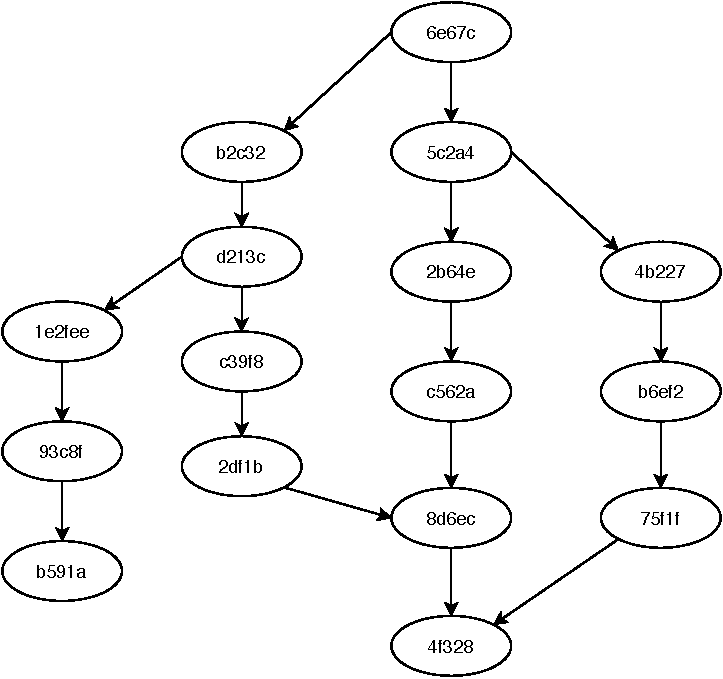
\includegraphics[width=\linewidth]{versiontree.pdf}
  \caption{基于修订关系的版本树示意图}
  \label{versiontree}
\end{figure}



CVS(Concurrent Versions System)是对RCS的进一步封装。在RCS的基础上,CVS实现了集中式的Client/Server架构应用,使得用户可以在多个终端下协同编辑代码,将代码更改提交到中心服务器上并追踪其内容变化。

SVN(Subversion)是对CVS的进一步优化。SVN实现了版本提交的原子化,在版本提交失败时,SVN不会保存任何提交的数据。SVN实现了对代码重构(包括文件名,文件目录组织等)场景的支持。同时,SVN的版本控制命令可以普遍应用于各类文件,包括所有Unicode和非ASCII命名的文本文件和所有二进制文件。集中式的版本控制系统受限于网络连接情况,并且中心服务器的故障会导致系统瘫痪。为了优化协同开发效率,分布式版本控制系统应运而生,代表如Git、Mercurial等。分布式版本控制系统在每一个终端都保留完整功能的代码仓库,使得开发可以在各个终端独立进行。

可以观察到上述演化过程中,版本控制系统面向传统软件开发过程演化的核心目标是优化代码协同开发过程的效率。由此演化出的版本控制基础即是RCS中提出的修订控制。虽然不同版本控制系统往往采用不同的修订策略(例如SCCS采用前向delta,RCS采用后向delta),但修订控制一直被沿用,并成为主流工具如SVN,Git,Mercurial的核心版本控制方法。

修订控制作为版本控制方法有许多优势。一方面,将修订组织为版本树,只需对部分版本保存完整内容,剩余版本只需存储到最近完整版本的修订,大大缩减了存储开销。另一方面,版本树追踪了文件的版本演化关系,这使得无论是本地、集中式还是分布式的版本控制系统中,不同用户提交的版本总是可以基于修订进行合并,便于维护数据一致性。

然而,基于修订的版本控制并不适用于二进制文件。一方面,对二进制文件的不同版本进行合并等操作可能导致潜在错误,例如在深度学习场景下,对不同版本的模型进行合并会导致未知的错误。另一方面,二进制文件的修订内容不具有可读性,例如在深度学习场景下,模型文件训练前后的数据变化无法直观反映模型训练时参数的调整,也无法直观体现模型性能的变化。

这使得主流的版本控制工具对于二进制文件的处理策略十分谨慎:Mercurial不支持对二进制文件进行内容追踪,仅存储其完整版本。Git提出Git-LFS作为二进制大文件追踪的解决方案。Git-LFS将对二进制文件生成一个指针,并将二进制文件区别于同一项目下的文本文件,用单独的服务器进行存储。Git-LFS的目的是解决在Git下保存二进制大文件时仓库体积庞大导致网络传输缓慢的问题。但Git-LFS并不能解决此问题,例如将二进制文件检出时,Git-LFS会通过指针获取文件内容,这意味着在检出时用户仍然要面临网络传输问题。Git-LFS同样不能解决解释性差和数据冗余问题。另外,由于二进制大文件的托管大量消耗服务器存储资源,使用Git-LFS的服务器需要面临严格的空间限制和并不便宜的价格。SVN对所有文件都进行字节粒度的内容追踪,通过特定的算法区分文本文件和二进制文件,并通过识别文件内容判断文件的上下文合并是否可行。但SVN用户依然需要自行判断是否需要对二进制文件进行追踪,并自行处理二进制文件内容追踪带来的问题。如在深度学习场景下,版本检出时将耗费大量计算资源从修订内容计算出指定版本。


\subsection{神经网络}
深度学习又称“神经网络学习”,深度学习的数据模型即神经网络模型。

“神经网络”是由具有适应性的简单单元组成的广泛并行互联的网络,它的组织能够模拟生物神经系统对真实世界物体作出的交互反应。神经网络可以视为包含了许多参数的数学模型,这个模型是由若干个函数相互嵌套而得。【机器学习】

神经网络的基本组成单元是神经元。神经元接收若干个输入信号(input),这些输入信号通过带权重(weight)的连接进行传递,神经元将所有的输入根据权重进行求和后传入神经元的激活函数(activation function),并产生神经元的输出(output)。典型的神经元数学模型如图\ref{neural},图中$i1$,$i2$表示$i3$分别神经元的三个输入,$w1$,$w2$,$w3$分别表示神经元三条输入连街边的权重,$o$表示神经元的输出,若用$f$表示神经元的激活函数,则神经元输出的计算过程为$o=f(i1*w1+i2*w2+i3*w3)$。许多神经元按照一定的层次结构组织起来就构成了神经网络。

\begin{figure}[htb]
  \centering
  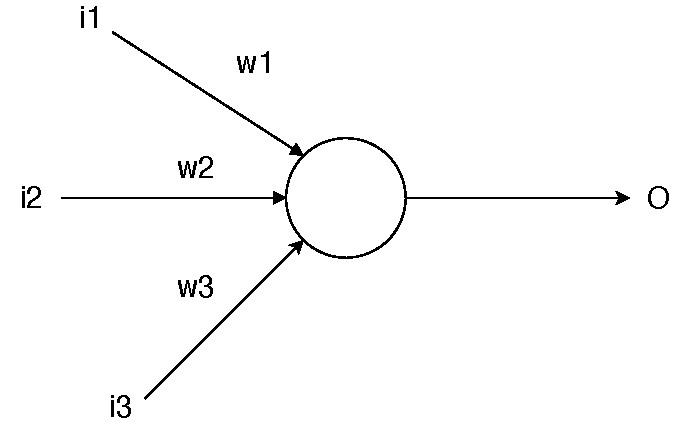
\includegraphics[width=\linewidth]{neural.pdf}
  \caption{神经元}
  \label{neural}
\end{figure}

常见的神经网络是层级结构,每层神经元与下一层神经元全连接,同一层神经元彼此不进行连接。图\ref{nn}中展示了典型的三层神经网络,其中包含一个输入层(input layer)和一个输出层(output layer),在输入层和输出层之间的层被称为隐层(hidden layer),在更复杂的神经网络中,往往有多个隐层。其中输入层接收外界输入,隐层与输出层神经元对信号进行加工,最终由输出层输出。神经网络的学习过程,就是根据训练数据来调整神经元之间的“连接权”,以及每个功能神经元的激活函数阈值。【机器学习】


\begin{figure}[htb]
  \centering
  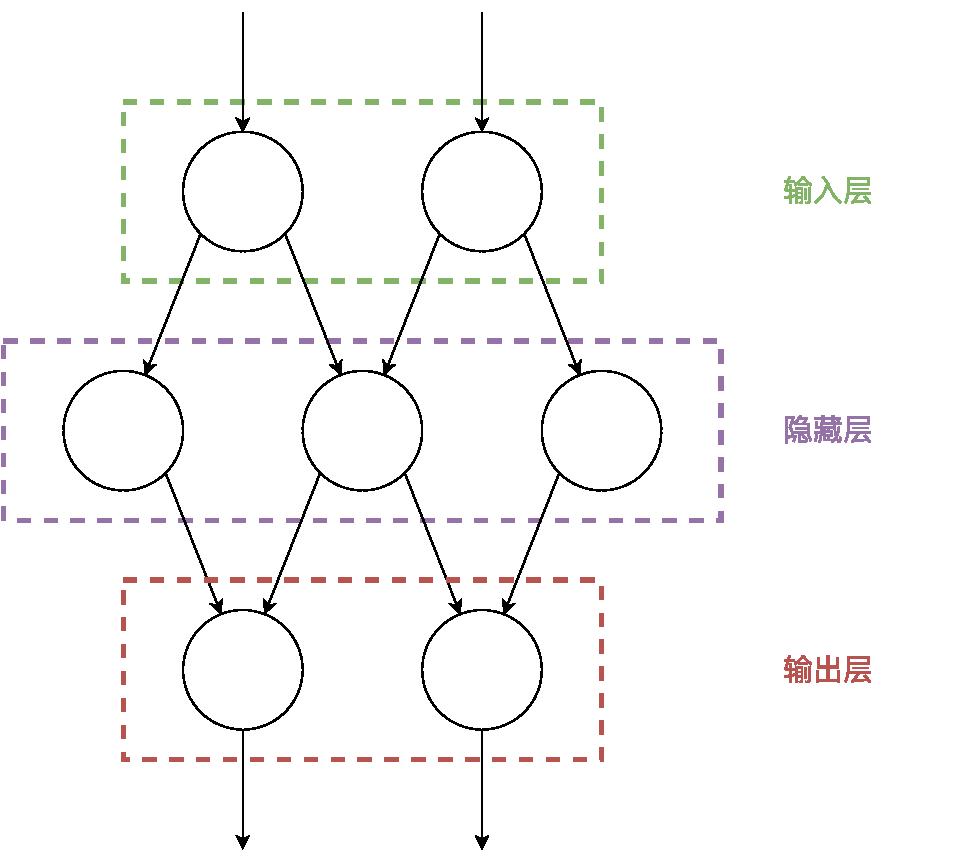
\includegraphics[width=\linewidth]{nn.pdf}
  \caption{三层神经网络}
  \label{nn}
\end{figure}


神经网络模型文件中的数据主要内容即是神经元之间的连接边的权重,称为模型权重。

从版本控制的角度看,区别于代码和配置等文本文件,神经网络模型是二进制大文件。一个神经网络模型通常包含大量的权重,权重通常为浮点数据,这使得单个神经网络模型通常需要占据数百MB的存储空间,这给神经网络模型的版本控制带来两方面挑战。一方面,神经网络模型文件内容为二进制数据,因此文件内容的追踪无法对模型内容变化进行直观反映。另一方面,由于训练前后神经网络模型权重被大幅度更新,以字节为粒度的修订追踪包含较高计算复杂度,从而影响检入检出粒度;以完整模型为粒度的版本追踪无法去除版本之间的冗余数据,导致存储开销快速增长;不存储模型文件则需要在检出所需版本时重新训练模型,由于模型训练过程耗时较大,不存储模型文件会为检出操作带来额外的时间开销。

\subsection{深度学习生命周期}
如图\ref{lifecycle}所示,一个典型的深度学习开发生命周期包含模型的创建、训练、评估和发布四个环节。

\begin{figure}[htb]
  \centering
  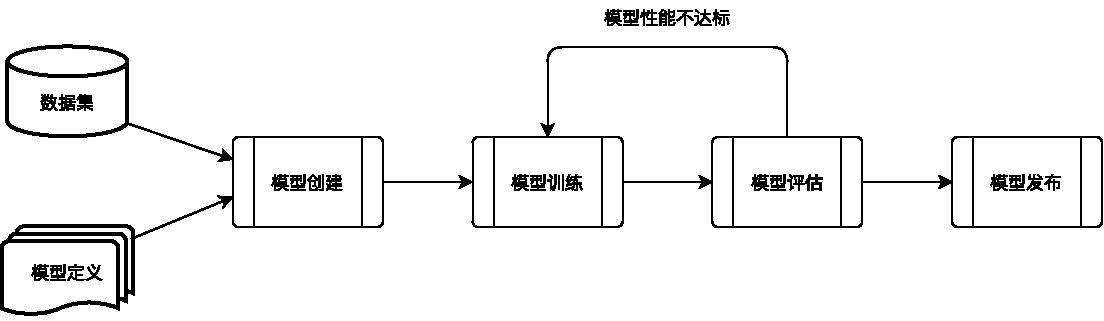
\includegraphics[width=\linewidth]{lifecycle.pdf}
  \caption{深度学习生命周期}
  \label{lifecycle}
\end{figure}

模型创建阶段,开发者通过定义模型的结构和初始化权重实现模型初始化。在进行模型结构定义时,开发者通常使用同类任务的优秀模型架构作为参考。在模型创建阶段,开发者还需要构建用于训练的数据集。更高质量的数据集往往能训练出性能更加的模型权重。由于高质量的数据集往往构建较为困难,开发者通常缺乏高质量的数据集,此时开发者通常复用在同类任务中在高质量数据集上表现出色的模型权重作为当前任务的模型权重初始值,并固定其中的部分权重不在后续过程更新以获取更好的模型性能(如固定特征提取层的权重则可以令模型获得更好的特征提取能力,因为这部分权重是在高质量数据集上训练所得)。

模型训练阶段,开发者设置一组训练配置(称为超参数),配置中通常包含迭代次数、损失函数、优化器等参数。模型训练过程中不断重复接收数据集,进行预测,计算损失函数,基于损失函数通过优化器更新模型权重的循环过程,直到迭代次数达到上限。流行的深度学习模型中通常包含大量的神经元,因此其模型的连接权和阈值数据量巨大,训练深度学习模型往往需要高额时间成本。

模型评估阶段,开发者通过对模型性能进行测试,判断模型性能是否达到期望。若达到期望则将模型发布,投入使用。否则调整模型训练的超参数或模型结构,重新回到训练环节。

模型发布阶段,开发者将模型部署,向外提供使用接口。

从深度学习的生命周期不难观察到,深度学习软件开发的核心是模型。开发过程的主要特征是对模型的反复训练、评估和调优。与传统软件开发过程相比,一方面,深度学习开发过程的版本控制无需多个终端参与。模型开发相较代码开发依赖于高性能的计算设备,且模型文件需要占用更大的存储开销,网络传输代价更高,因此深度学习软件开发过程通常在同一个主机或计算机集群上进行。另一方面,深度学习开发过程的版本控制无需多个用户参与。模型开发的核心是模型迭代,相关代码通常量较少且迭代较少,因此模型开发的主体流程中通常不涉及多个用户对模型或其相关文件进行频繁修改。

\section{系统设计与实现}
深度学习软件开发的核心是模型,其开发过程的主要特征是对模型的反复训练、评估和调优。与传统软件开发过程相比,深度学习软件开发过程协同性较低,其版本控制通常无需多个终端或多个用户参与。

因此,深度学习友好的版本控制是本地模式的版本控制,其核心并非多用户协同,而是在频繁的模型迭代过程中提供具有良好可读性的版本追踪方法以及通过合理粒度的存储管理策略在存储开销和检入检出性能间达成平衡。

本文基于上述观察设计并实现了以模型为核心的版本控制工具NNTracer。NNTracer在模型训练过程中基于模型“元信息”进行版本追踪。同时,NNTracer以“层”为粒度对模型文件进行存储管理以减少存储开销并确保检入检出性能。

\subsection{版本追踪模块}
版本追踪的目的是为用户提供具有良好可读性的版本历史描述,令用户可以基于版本追踪内容对历史版本进行分析,并在需要的时候选择特定的历史版本检出进行查阅。传统版本控制工具基于文件内容的修订进行版本追踪,但这种方式对深度学习模型开发并不适用。基于上述现象,本文提出基于深度学习模型的“元信息”进行深度学习开发过程的版本追踪。

\subsubsection{深度学习模型的元信息}
版本控制是对文件的历史版本追踪。版本控制工具对每一个历史版本记录其变更内容,从而标记一个历史版本。开发者通过查看历史版本的变更内容即可对历史版本进行分析,或选择某个历史版本进行检出。因此,历史版本的变更内容以人类可读的方式被记录是开发者后续分析和选择特定历史版本的基础条件。

在传统软件开发过程中,文本文件的修订既是文件内容变更的直接体现,也具备良好的人类可读性。然而,在深度学习开发过程中,基于修订对模型进行追踪时产生的文件修订并不具有人类可读性,如图\ref{modelrevision}所示。

\begin{figure}[htb]
  \centering
  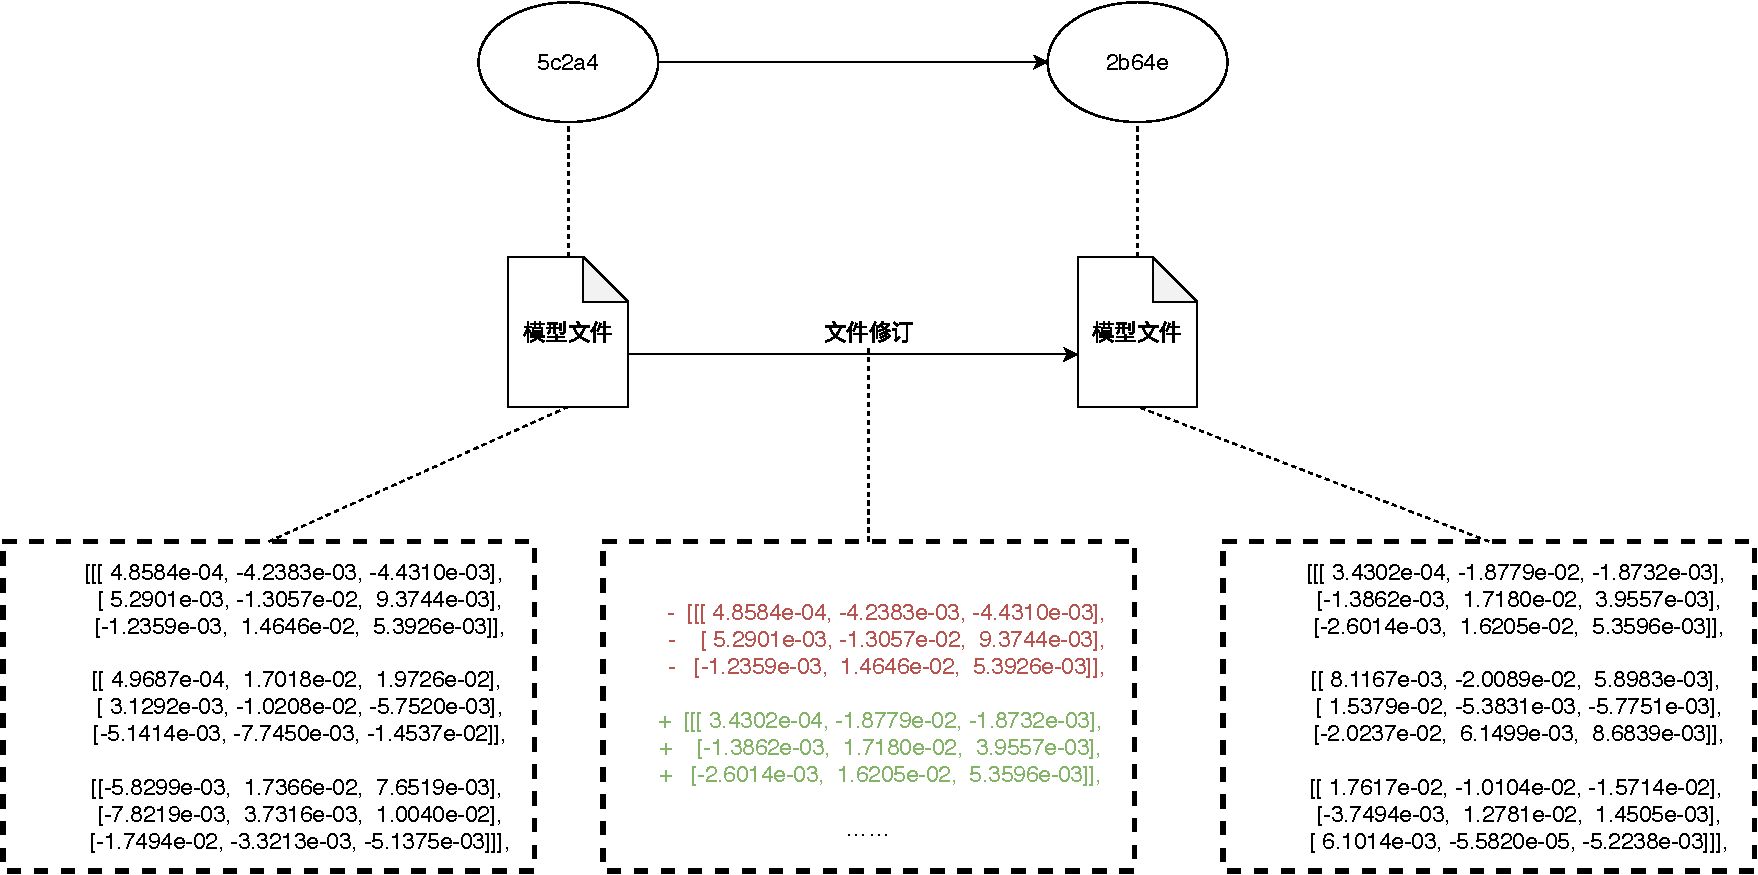
\includegraphics[width=\linewidth]{modelrevision.pdf}
  \caption{模型文件内容变更}
  \label{modelrevision}
\end{figure}

虽然深度学习模型的文件内容修订无法对其内容变更进行人类可读的描述,但深度学习模型的内容变化是由模型的训练配置、模型结构等因素的变化而导致的。这些信息既可以用于复现一个版本的模型,也可以以文本的形式记录一个版本中模型的变更,从而实现具有人类可读性的版本追踪。本文提出“元信息”的概念用于描述这类信息。

\begin{definition}
元信息:能够复现文件的某个版本的全部信息的总和。
\end{definition}


传统软件开发过程的核心是代码。开发过程的主要特征是对代码的协同和频繁修订。在代码开发过程中,对代码文件的修订可以复现指定版本,因此代码的修订可以定义为一个版本代码的“元信息”。

深度学习软件开发的核心是模型。开发过程的主要特征是对模型的反复训练、评估和调优。在模型训练过程中,开发者需要设置训练配置和模型结构,例如设置合理的损失函数和优化器,模型中各个层的输入输出尺寸等,在训练结束后,开发者会得到经过训练的模型权重。在模型评估的过程中,开发者需要在测试集上验证模型的性能并记录。在模型调优时,开发者基于模型评估的结果对训练配置和模型结构进行调整以取得更好的效果。模型的训练即是上述三个过程的不断迭代,其训练过程由代码文件进行控制。本文将上述过程涉及的模型结构、模型权重、训练配置、评估结果和代码文件信息的总和定义为深度学习开发过程的“元信息”。

\subsubsection{基于元信息的版本追踪}
从前文中不难看出,在“元信息”中,通过模型结构和模型权重可以高效地复现一个版本的模型文件,但一方面模型结构和权重通常并不包含项目版本中的其他可用于分析的必要信息,如评估结果等;另一方面模型权重的存储需要占用大量空间。训练配置、评估结果和代码文件无需占用过高的存储空间,且可以复现一个版本的深度学习项目的完整内容,但为了复现对应版本的模型需要对模型进行重新训练,从而需要高额时间成本。事实上,“元信息”中可以用于复现项目版本的信息最小集仅包括训练配置、评估结果和代码,但仅保存此最小集无法实现高效的检入检出,因此模型结构和模型权重依然是”元信息“中的重要元素。

对深度学习开发过程进行版本追踪,实质是对“元信息”的版本追踪。传统的版本控制工具通过对静态文件修订的计算得到一个版本的“元信息”。但一方面从二进制大文件中提取模型的“元信息”是困难的,另一方面不同的模型架构和不同的模型评估标准会令训练配置和评估结果的数据结构大相径庭,这使得被写入文件的元信息通常是非结构化的,且通常是经过开发者筛选的。尽管可以通过静态分析的方式从代码等相关文件中提取“元信息”,但对静态文件的分析过程需要一定时间开销且存在错误的风险。更重要的是从静态文件中提取模型的“元信息”是反直觉的,因为模型的“元信息”总是完整地存在于运行时刻,开发者对模型数据的存储和读取也总是在运行时进行。

由此,NNTracer提出了与Git,SVN等工具截然不同的版本检入方式,即运行时的版本检入。NNTracer提供基于深度学习框架的版本检入接口,开发者通过在运行时调用版本检入接口对运行时存在的模型“元信息”进行检入。

NNTracer的版本检入工作流如图\ref{checkin}。

\begin{figure}[htb]
  \centering
  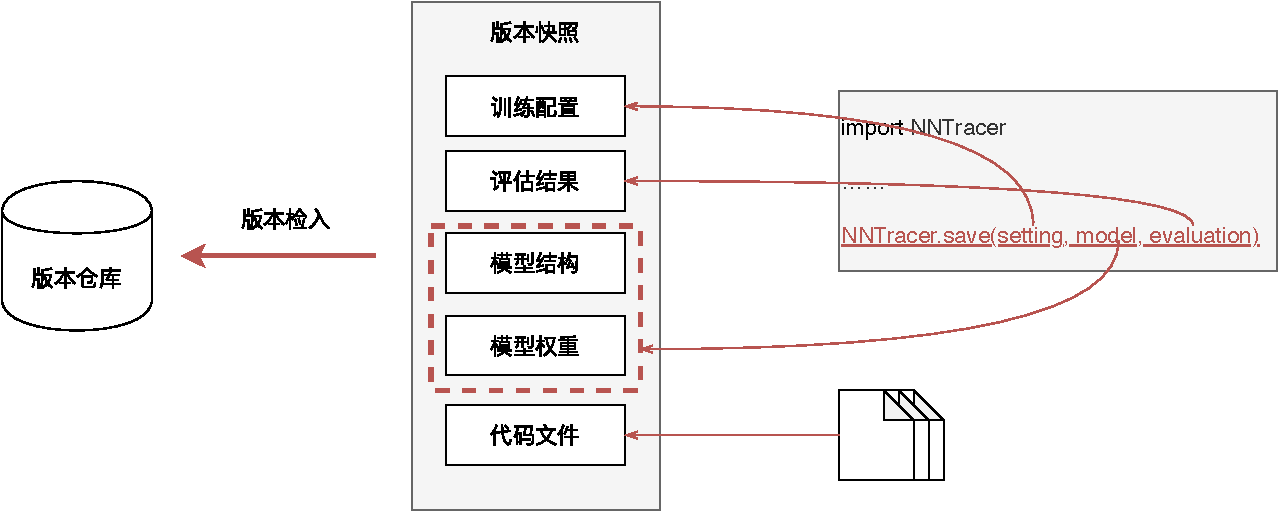
\includegraphics[width=\linewidth]{checkin.pdf}
  \caption{NNTracer版本检入工作流}
  \label{checkin}
\end{figure}

开发者通常基于深度学习框架查看模型结构和模型权重,例如PyTorch的模型结构和模型权重分别可以通过类实例的\_\_str\_\_和state\_dict方法获取。NNTracer提供基于深度学习框架的版本检入接口实现对指定框架下模型的结构和权重信息抽取。对于PyTorch框架,开发者只需在调用PyTorch框架下的NNTracer检入接口时传入模型实例即可实现模型结构和模型权重的抽取。

开发者通常通过日志输出运行时刻的训练配置和评估结果。正如前文所述,不同的模型架构和不同的模型评估标准会令训练配置和评估结果的数据结构大相径庭。由此,NNTracer仅对检入接口的训练配置和评估结果参数进行宽松的格式检查,开发者只需提供符合JSON语法的训练配置和评估结果。

在运行时刻,深度学习项目的代码不会被修改。NNTracer在检入接口被调用时扫描当前深度学习项目中的代码文件形成文件快照,并对代码的文件快照进行版本追踪。

NNTracer抽取上述“元信息”后组织为人类可读的版本快照,并生成唯一的id作为版本标识。通过版本标识,开发者可以对指定版本进行检出。

NNTracer提供两种版本检出方式:运行时检出和命令行检出。

NNTracer的版本检出工作流如图\ref{checkout}。

\begin{figure}[htb]
  \centering
  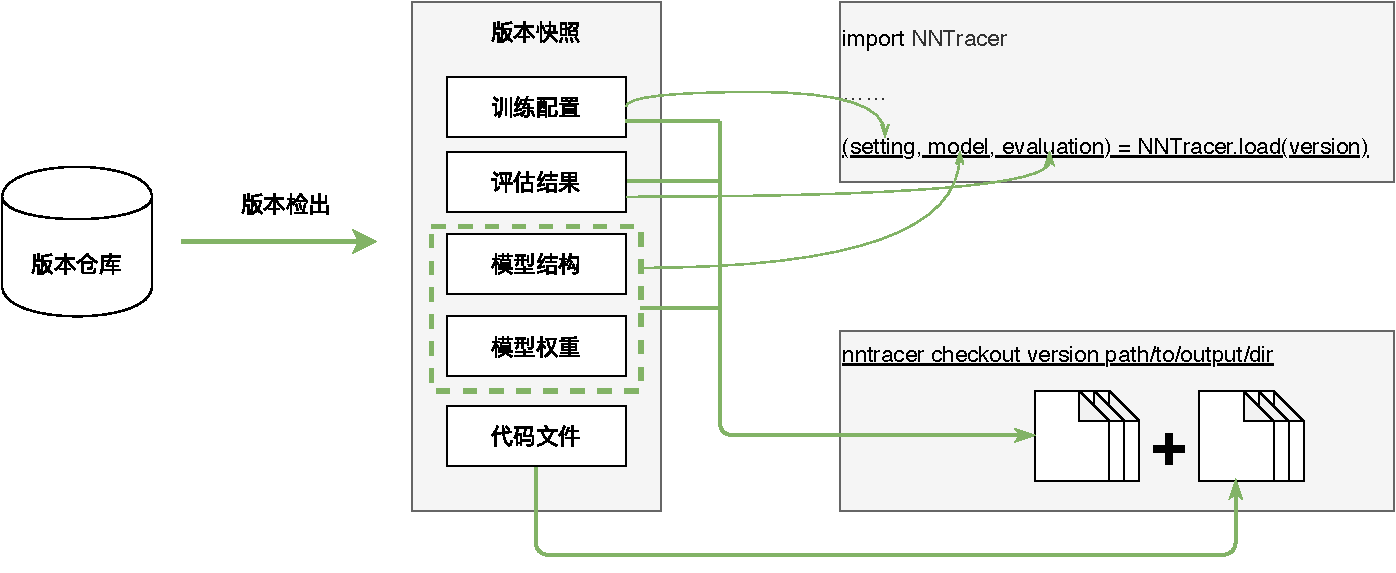
\includegraphics[width=\linewidth]{checkout.pdf}
  \caption{NNTracer版本检出工作流}
  \label{checkout}
\end{figure}

运行时,开发者通常需要加载指定版本的模型并进行训练配置或模型结构调整。NNTracer提供指定深度学习框架的版本检出接口,开发者通过传入版本标识获得由模型权重、训练配置和评估结果信息构成的元组。

对历史版本分析时,开发者通常需要检出完整的历史版本信息。NNTracer提供命令行工具,开发者通过调用命令行指令,传入版本标识和检出路径,即可将指定版本的深度学习项目检出到指定路径。

\subsection{存储管理模块}
版本控制的存储管理目标是保持检入检出高效的情况下尽可能降低总存储开销。在深度学习的场景下,模型在随版本演化过程中不可避免地产生冗余数据。基于上述现象,本文提出以层为粒度的存储管理以减少冗余数据导致的额外存储开销。

\subsubsection{深度学习开发过程的冗余数据}
深度学习开发过程中的冗余数据主要来自两个方面:重复被存储的模型权重和无需被存储的模型版本。

一方面,当开发者固定了模型当中的部分权重,不在后续的训练过程中更新时,该部分权重会被后续版本的模型所包含,从而被重复存储。另一方面,开发者常常会训练大量版本的模型,其中只有少部分较为成熟或更具备参考价值的模型会在后续的开发过程中被多次检出和分析,对于开发者在后续过程中大概率不会检出的版本,保存该版本的模型文件会造成不必要的存储开销。

在进行深度学习开发时,开发者通常通过迁移学习构建模型或从头开始构建模型,然后对模型进行反复训练、评估和调优。无论开发者如何构建模型,都会不可避免地形成上述两种情形的额外存储。

从头开始构建模型的训练过程是成本较高的。由于模型权重的初始值是随机的,为了令模型权重达到收敛,训练时间往往需要持续数小时到数日,其中通常包含大量无需进一步分析的模型版本,只有少数版本的模型权重需要被记录和保存。对于已经收敛的权重(如特征提取部分的权重)开发者常常会在后续的开发中将其固定,不进行权重更新,以降低训练时间成本。

通过迁移学习构建模型时,开发者选择同类任务中性能优秀的模型作为模型的初始权重,固定其中部分权重,在后续的开发过程中不对该部分权重进行更新。这样的做法有许多好处,一方面,深度学习开发中常常缺乏足以训练出优秀模型的高质量数据集,通过复用同类任务中在高质量数据集上训练出的模型参数,可以弥补数据集的不足,提高模型性能,例如在图像识别任务中,复用在ImageNet数据集上表现优异的模型权重可以有效提高模型的特征提取能力。另一方面,通过固定被复用的模型权重,可以大大减少模型需要更新的权重数量,从而大大缩短训练所需的时间,提高开发效率。

冗余数据产生的根本原因是模型训练成本过高,导致开发者需要保存训练好的模型以用于后续的分析。因此,良好的存储管理需要确保模型分析过程的检入检出性能,同时尽可能减少模型随版本演化过程产生的冗余数据。

\subsubsection{以层为粒度的存储管理}
对冗余数据进行检测和消除,关键在于选择合理的粒度。粒度越大意味着冗余消除的效果越差,但冗余检测的过程随之大幅简化。当粒度减小,检测冗余的复杂度会大幅上升,但冗余消除的效果随之提高。例如,当调用深度学习框架的保存接口对模型进行保存时,不同版本的模型均保存为独立的文件,此时存储开销为所有版本模型的总体积之和,但此时完全没有冗余检测的过程,保存过程效率很高。当使用SVN对多个版本的模型进行打包时,模型的总存储开销显著减少,但由于SVN使用字节粒度的算法计算文件修订,因此打包过程运算量极大,需要对应的时间成本和内存开销。【参考文献】

深度学习模型中,模型权重被封装为若干个相互连接的层。在设置模型结构时,开发者通常以层为单位选择需要固定不更新的参数以及需要更新的参数。因此模型的权重总是以层为粒度被复用,并总是以层为粒度被更新。权重的复用以层为粒度进行,这意味着被复用的层所有的权重总是不会被更新。权重的更新以层为粒度进行,这意味着被更新的层所有的权重总是同时被更新。由此,本文提出以层为粒度的存储管理,即将模型权重以层为粒度进行分割,并在多版本间进行冗余检测,避免以层为单位的数据被重复存储。

当模型结构和模型权重被检入时,NNTracer首先根据模型结构将模型权重按层分割为若干向量,然后对各个向量计算其哈希值,并尝试将向量和对应的哈希值存入版本数据库。如果哈希值没有冲突,则该层并未被复用,可以直接存储;反之则将哈希值冲突的两个向量做差,若结果为0向量,则意味着该层被重复存储,此时抛弃新提交的层,仅保留已存在的层;若做差后结果为非0向量,则意味着该层未被重复存储,此时NNTracer对当前检入的层哈希值进行微调并重新检入。

针对无需进一步分析和检出的模型权重,NNTracer提供从指定版本中移除模型权重的存储管理功能。NNTracer提供命令行接口,接收指定版本标识作为输入,开发者调用接口移除指定版本的模型权重。当接口被调用时,NNTracer检测版本数据库中该模型包含的层,对于未被复用的层,NNTracer直接进行删除;对于被其他版本模型复用的层,NNTracer不进行任何操作。

\subsection{系统实现}
本文设计并给出了基于PyTorch和Linux环境的NNTracer实现。其系统架构如图\ref{architecture}。

\begin{figure}[htb]
  \centering
  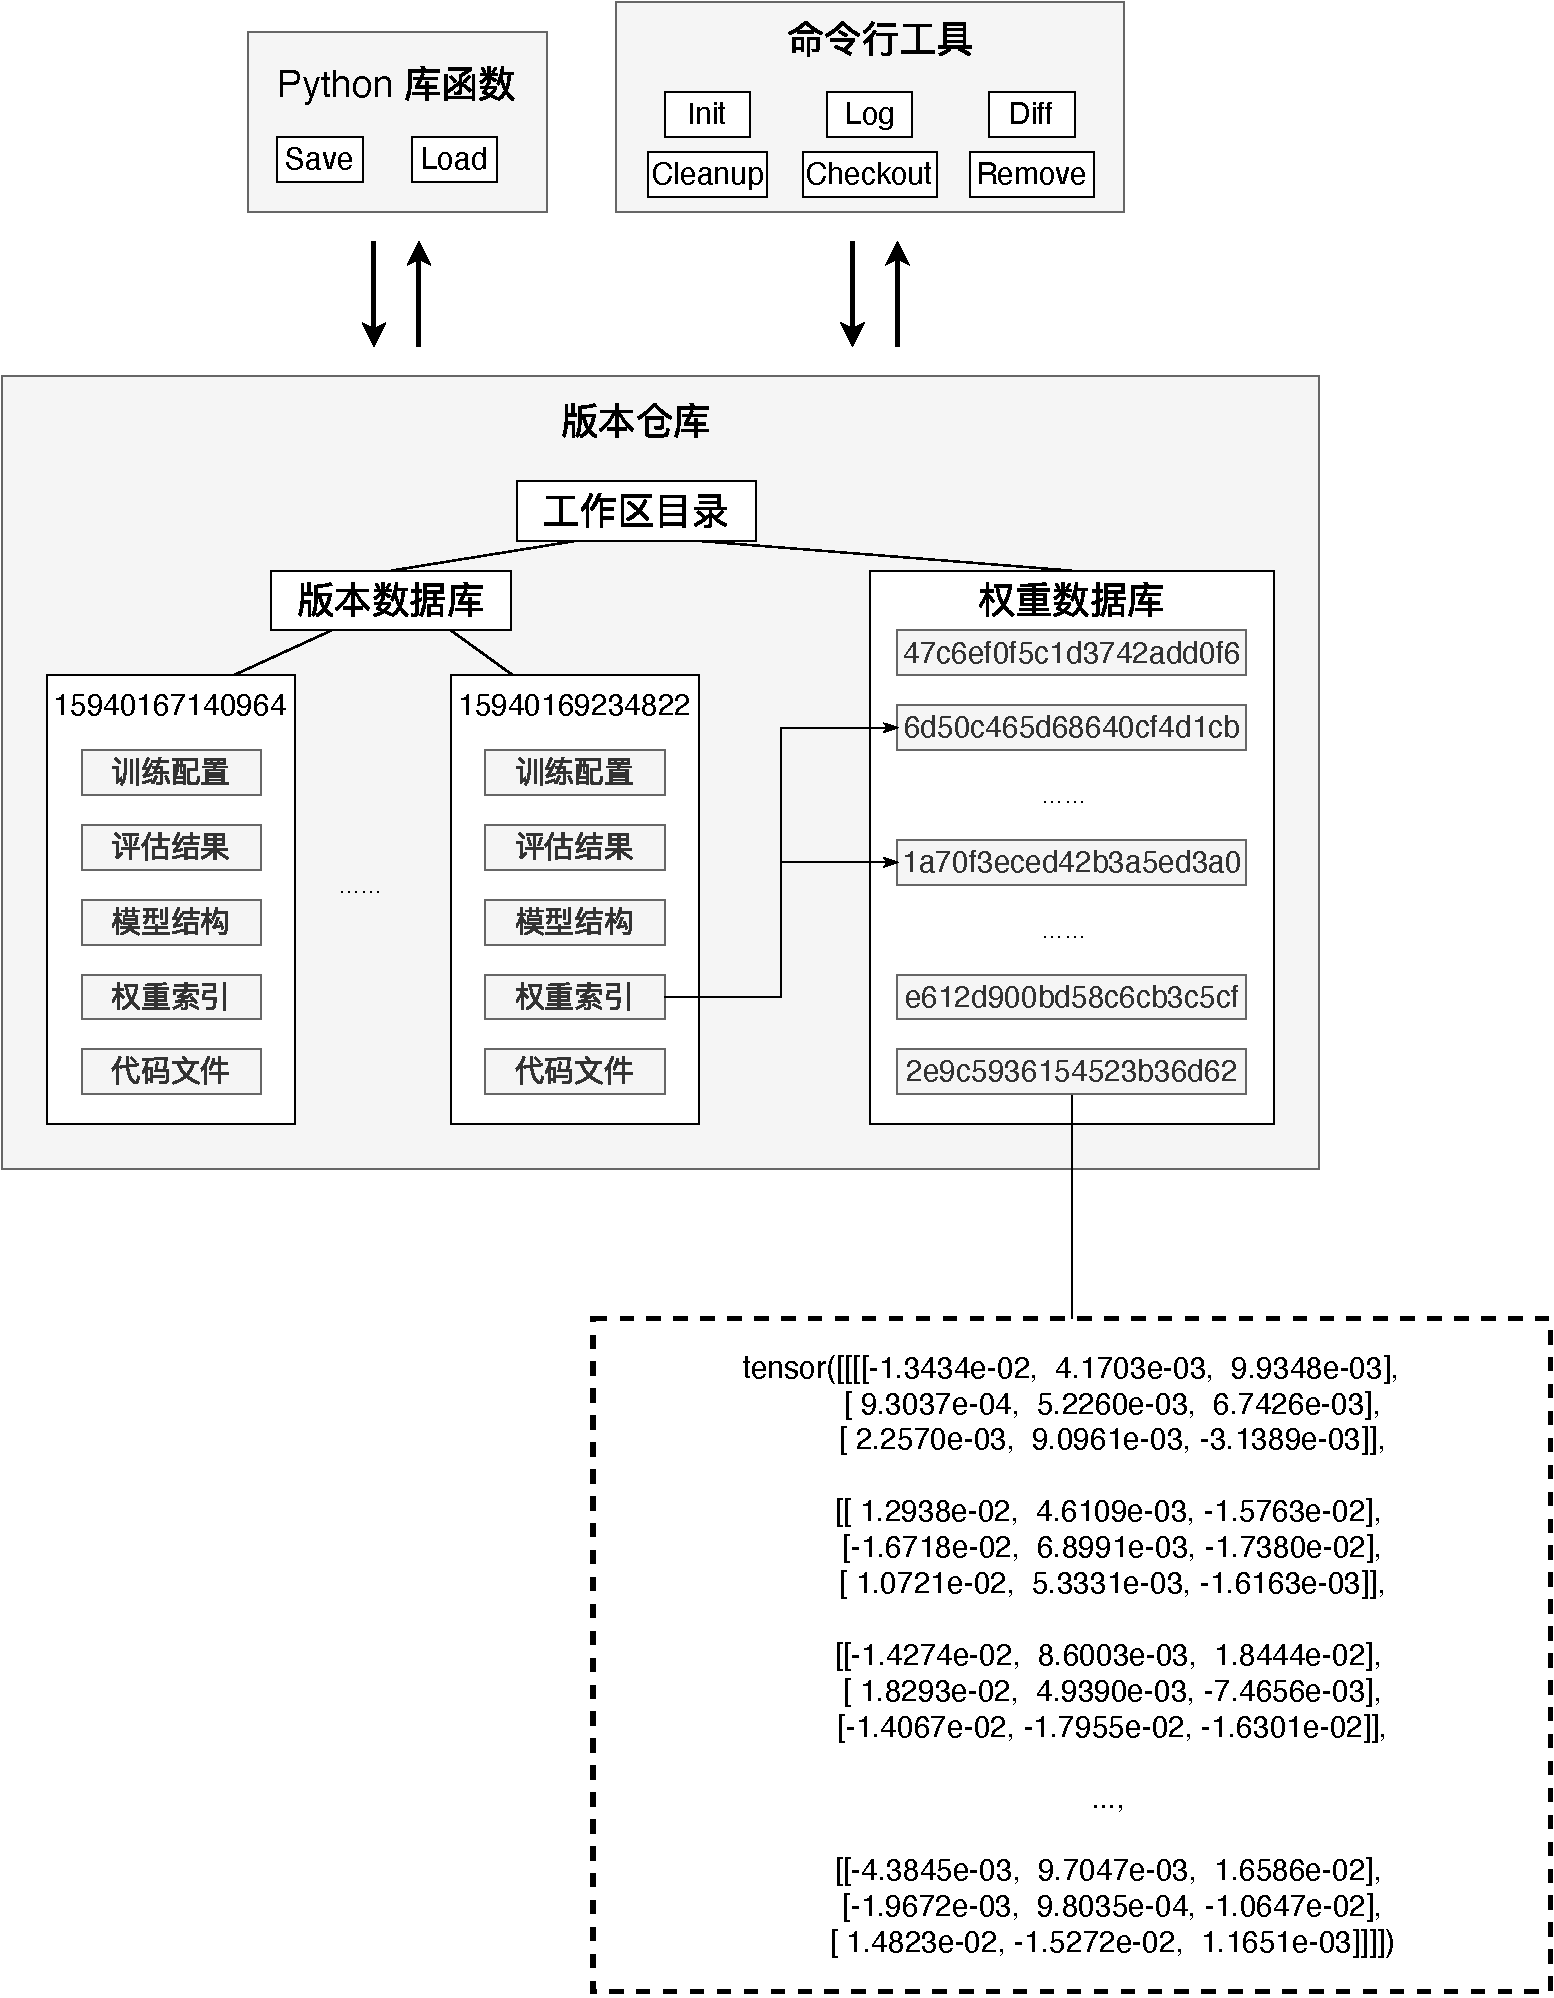
\includegraphics[width=\linewidth]{architecture.pdf}
  \caption{NNTracer系统架构}
  \label{architecture}
\end{figure}

和其他版本控制工具类似,NNTracer通过版本仓库管理深度学习项目的各个版本。仓库独立地维护深度学习项目中的各个版本。开发者可以在任意目录下初始化一个仓库,该目录随即被仓库管理员标记为一个深度学习项目的根目录。仓库包含项目的版本数据和用于管理数据的接口。

在NNTracer的仓库中,深度学习项目的版本数据被组织为一颗文件树。其根结点为开发者初始化仓库时在深度学习项目根目录下创建的工作区目录。在工作区目录下,所有版本的数据被划分为权重数据库和版本数据库,分别对应两个子目录。

权重数据库以键值对的形式存放所有版本的权重数据:全部版本的模型权重按层分割,每一层都以哈希值为标识符被存放。在基于PyTorch的NNTracer实现中,NNTracer首先调用PyTorch的接口(\_\_str\_\_)对层的权重数据进行采样并字符串化,然后使用Sha1算法对字符串计算哈希值。权重数据库中的层有引用数量字段,该字段标记了包含当前层的模型版本数量。

版本数据库中以键值对的形式存放各个版本的元信息,每一个版本都以版本号为标识被存放。每个版本中包含该版本对应的训练配置、评估结果、代码、模型结构和模型权重索引。其中,模型权重索引是用于在权重数据库中查询该版本权重数据的索引文件。在本文的实现中,NNTracer基于unix时间戳生成版本号。

开发者通过接口对仓库进行管理。NNTracer提供两类接口:提供项目管理功能的命令行工具和提供运行时版本检入检出功能的库函数。

命令行工具提供用于对仓库进行管理的若干指令。在本文的实现中,NNTracer的命令行工具提供命令行环境下版本控制的所有必要指令:init、cleanup、log、checkout、remove和diff。

init命令将当前目录标记为一个深度学习项目,并在当前目录下初始化NNTracer仓库,创建仓库对应的目录结构、模型数据库和版本数据库。

cleanup命令通过当前工作目录检测当前深度学习项目,清理该项目下的所有仓库数据,并移除对该项目的标记,取消对该项目的版本追踪。

log命令通过当前工作目录检测当前深度学习项目,从最新的版本开始按时间序打印版本记录,每一条记录包含该版本的模型结构、训练配置和评估结果的文本信息。

remove命令通过当前工作目录检测当前深度学习项目,并接收版本号作为参数,移除该深度学习项目中对应版本的权重文件。NNTracer首先根据版本号查询该深度学习项目版本数据库中的模型权重索引。根据模型权重索引在权重数据库中检索该版本模型包含的各个层,对于引用数量为1的层,表示当前层仅被即将删除的版本包含,此时直接删除该层权重数据;对于引用数量不为1的层,表示当前层被多个版本的模型包含,此时不删除当前层的数据。对权重数据库处理完毕后移除版本数据库中该版本的模型索引文件。

checkout命令通过当前工作目录检测当前深度学习项目,并接收版本号和检出路径作为参数,将该深度学习项目中对应版本的文件检出到指定路径。首先,NNTracer根据版本号从该深度学习项目的版本数据库中读取该版本的训练配置、评估结果、代码、模型结构和模型权重索引。随后,若模型索引不为空,NNTracer根据模型权重索引从权重数据库中读取各个层的权重数据,并按照模型结构将独立的层数据组织为完整的模型权重数据,并将训练配置、评估结果和模型权重写入到文件,并和该版本的代码一同写入到检出路径。若模型索引为空,则目标版本的模型权重已被删除,此时仅将训练配置和评估结果写入到文件,并和该版本的代码一同写入到检出路径。

diff命令通过当前工作目录检测当前深度学习项目,并接收两个版本号作为参数,读取该深度学习项目中的两个版本数据并输出对比结果。NNTracer分别用两个版本号查询版本数据库中对应版本的训练配置、模型结构和评估结果。并通过diff算法对上述文本内容进行对比,输出其结果。

库函数模块提供基于深度学习框架(如TensorFlow,PyTorch,Keras等)的版本检入和检出功能。在基于PyTorch实现的NNTracer中,库函数以Python包的形式提供简洁的接口调用:save和load。

save接口接收开发者传入的训练配置、模型实例(PyTorch下的nnModule类实例)和评估结果作为参数,获取模型元信息并检入到仓库。在接收到参数后,NNTracer使用PyTorch框架下的nnModule类方法导出模型实例中的模型结构和模型权重信息。随后,NNTracer将模型权重按照模型结构分割为若干层,并将权重数据提交到权重数据库,获取模型权重在权重数据库中的索引文件。同时,NNTracer获取当前深度学习项目中的代码文件快照。最后NNTracer将训练配置、评估结果、代码、模型结构、模型权重索引提交到版本数据库。

load接口接收版本号为参数,读取仓库中开发者需要检出的数据并返回。在接收到参数后,NNTracer从版本数据库中读取版本号对应的训练配置、评估结果、模型结构和模型权重索引。随后,若权重索引不为空,NNTracer根据模型权重索引从权重数据库中读取各个层的权重数据,并按照模型结构将独立的层数据组织为完整的模型权重数据。若权重索引为空,则当前版本模型权重已被删除,此时将模型权重数据标记为空值。最后,NNTracer将训练配置、评估结果和模型权重文件构成的元组返回(在PyTorch中,开发者通常只保存和读取模型的权重)。

\section{实验与评估}

本章节中对NNTracer的版本控制过程中以层为粒度的存储管理方法进行性能评估。

本实验以如下深度学习开发项目为场景:基于使用ImageNet预训练的卷积神经网络模型进行调优,实现猫狗图片二分类模型。ImageNet项目是一个用于视觉对象识别软件研究的大型可视化数据库。通常在ImageNet上预训练的模型可以对图片特征进行良好的提取。卷积神经网络通常包含若干卷积层和若干全连接层。其中卷积层部分用于提取数据特征,全连接层部分用于对数据特征进行分类。在实际开发中,开发者通常复用在高质量数据集上预训练的卷积层以有效地提取图片特征,然后根据实际任务对全连接层进行部分或全部重新训练来达到更好的分类效果。

为了评估NNTracer在规模不同的模型下的性能,本实验分别在Restnet18和Vgg16模型上进行性能评估实验。Resnet18模型包含5个卷积模块和1个全连接层,PyTorch框架的预训练模型体积为50M。VGG16模型包含5个卷积模块和3个全连接层,PyTorch框架的预训练模型体积为513M。

具体地,本实验设置4个分组,如表\ref{expgroup}:
\begin{table}
\caption{实验分组设置}
\label{expgroup}
\begin{center}
 \begin{tabular}{| m{1cm} | m{6cm} |} 
 \hline
 序号 & 训练方法 \\ 
 \hline\hline
 r1 & 固定Resnet18的其他层,仅对全连接层重新训练 \\ 
 \hline
 v1 & 固定Vgg16的其余层,仅对最后1个全连接层重新训练 \\
 \hline
 v2 & 固定Vgg16的其余层,仅对最后2个全连接层重新训练\\
 \hline
 v3 & 固定Vgg16的其余层,仅对最后3个全连接层重新训练  \\ 
 \hline
\end{tabular}
\end{center}
\end{table}

在以层为粒度的版本存储方法下,被复用的权重不会被重复存储。在此场景下,仅有第一次检入时会提交完整的模型文件,此后每次检入仅提交被重新训练层的权重,即每次训练后模型总存储的增量为定植。因此,模型文件的存储占用量与检入次数成线性关系,进行少量训练即足以验证存储开销的增长趋势。本实验分别对Restnet18和Vgg16模拟10次训练。在每次训练完成后对模型进行保存。在10次训练完成后,分别在命令行和运行时对模型进行100次随机版本检出。并统计每个分组模型的平均检入时间,在命令行和运行时分别的平均检出时间和十次训练后总存储开销。

作为对照组,本实验通过PyTorch的官方序列化接口在每次训练结束后对模型进行存储,并统计其模型存储和读取100次所需的平均时间,以及十次训练后的总存储开销。由于PyTorch以模型为粒度进行存储,在本实验中模型总参数量不变,因此v1,v2,v3的不同策略不会导致对照组的性能指标有所区别。故本实验中区分Resnet18和Vgg16,设置2个对照组,如表\ref{refgroup}。
\begin{table}
\caption{实验对照组设置}
\label{refgroup}
\begin{center}
 \begin{tabular}{| m{1cm} | m{6cm} |} 
 \hline
 序号 & 训练方法 \\ 
 \hline\hline
 rp & 用PyTorch序列化接口进行版本管理 \\ 
 \hline
 vp & 用PyTorch序列化接口进行版本管理 \\
 \hline
\end{tabular}
\end{center}
\end{table}



\section{相关工作}

开源社区中,存在对深度学习过程提供数据管理支撑的工具。代表性的有sacred,torchtracer和mlflow等。

sacred是用于记录机器学习实验的开源工具。sacred通过代码中的注解区分模型训练的配置和运行脚本。并将训练配置和结果保存至mongodb。在检出时,用户可以通过命令加载脚本和配置重新生成某个版本的模型。sacred可以为实验分析提供丰富的历史记录,同时由于仅保存训练的超参数和结果,并不保存模型本身,从而不会对存储产生过多负担。但在想要检出某个版本的模型时,需要通过对应版本的配置和训练脚本对模型重新训练。在深度学习场景下,检出一个模型需要面临从初始状态训练模型的高额时间成本。

torchtracer是基于PyTorch框架的模型训练记录工具。torchtracer需要用户在代码中创建实例,并通过该实例的接口存储超参数、运行结果和模型文件。torchtracer可以记录深度学习开发过程的大部分数据,这避免了开发者的对不同的项目重复编写用于记录信息的代码。但torchtracer中同时需要用户通过文件命名来区分保存的不同版本的模型和配置,版本管理仍然依赖于开发者。同时由于torchtracer并不保存训练时的脚本,因此可能存在模型文件和变更后的训练脚本版本不一致的问题。

mlflow是一个开源的机器学习生命周期管理平台。它并非面向版本控制的平台,但提供机器学习模型追踪组件。其中,模型追踪以每一次运行为单位。在运行结束后,用户可以选择记录脚本对应的Git版本号,运行的起始终止时间,并可以选择通过键值对存储开发者选择的超参数,或记录任意类型的数据,如损失函数的收敛轨迹,模型文件等。mlflow具备相对完善的模型追踪功能。但mlflow下模型的存储仍然是以存储整个模型为粒度,因此无法规避额外存储开销。同时,mlflow的模型追踪需要在代码中插入大量mlflow的接口调用以实现对模型生命周期更全面的管理,这使得mlflow具有相对高的学习成本。

\section{总结与展望}

本文分析了现有版本控制工具在深度学习场景下的局限,提出了深度学习友好的版本控制工具NNTracer的设计与实现。为了对深度学习开发的版本控制进行全方位的支持,NNTracer仍有局限和不足,这些也是下一步工作改进的方向。

一方面,虽然NNTracer对本地模式的深度学习开发过程可以提供版本追踪和存储管理功能,但对于模型的发布和共享尚未提供足够的支持。模型的发布和共享是深度学习模型生命周期的环节之一,其过程需要涉及模型数据的网络传输。由于模型文件通常体积较大,发布和共享过程在传输速度方面可能会遇到挑战。

另一方面,本文仅给出了NNTracer的通用架构,并基于PyTorch做了基础实现。其中版本数据库和模型数据库均为通过文件系统进行简单实现,事实上,通过使用更高性能的数据库,可以进一步提升NNTracer的检入检出性能。但替换成其他组件实际上增加了NNTracer对其他软件的依赖,同时也需要对不同的数据库组件进行适配。无论是基于文件系统实现更适合深度学习开发的数据库,或是将现有的数据库应用到NNTracer框架中,都是可能的性能优化方向。

最后,虽然NNTracer提出以层为粒度进行存储管理的方式来消除冗余数据,但对模型版本是否需要保存,仍然交给开发者进行判断。这个过程或许可以通过一些策略和算法来代替开发者进行更加自动化的模型删除,如定时淘汰时间戳最早版本的模型文件。或是通过机器学习、模式识别辅助开发者进行判断,如通过评估结果判断当前模型是否欠拟合或过拟合。


\begin{figure}[htb]
  \centering
  \includegraphics[width=\linewidth]{example-fig.pdf}
  \caption{图片说明 *字体为小 5 号,图片应为黑白图,图中的子图要有子图说明*}
\end{figure}



\begin{acknowledgments}
  致谢内容。
\end{acknowledgments}


\nocite{*}

\bibliographystyle{cjc}
\bibliography{example}


\newpage

\appendix

\section{}

附录内容置于此处,字体为小5号宋体。附录内容包括:详细的定理证明、公式推导、原始数据等


\makebiographies


\begin{background}
*论文背景介绍为英文,字体为小5号Times New Roman体*

论文后面为400单词左右的英文背景介绍。介绍的内容包括:

本文研究的问题属于哪一个领域的什么问题。该类问题目前国际上解决到什么程度。

本文将问题解决到什么程度。

课题所属的项目。

项目的意义。

本研究群体以往在这个方向上的研究成果。

本文的成果是解决大课题中的哪一部分,如果涉及863/973以及其项目、基金、研究计划,注意这些项目的英文名称应书写正确。
\end{background}

\end{document}
